\section{Straight running}
%
The first developed example which is the simple straight running starting from a condition of steady state, the one calculated in chapter \ref{Ch:SS}. In this example the motorcycle travel along a straight line of fixed length in minimum time. It starts from the above mentioned steady state, accelerate and then brake to finish with the same velocity of the starting point.\\
This example could seem trivial, but it is a necessary step to validate the model.
%
\subsection{Solution approach}
%
This is the most straightforward example that can be think of for a minimum time optimal control. For this reason there is no need for special precautions or convoluted strategies to solve the problem. However, even in this case, the author chose to use the continuation technique to first solve a problem tracking the steady state. In a second time the minimum time is pushed while the steady state is cancelled. Then also the constraints on the maximum slips are pushed at lower values.\\
Setting the initial and final condition could be difficult. In particular some problem arise if too many initial condition are given because they cannot be feasible all together. Another problem appears if some conditions are left free. For instance if the height $h$, rear and front suspension $\theta$ and $s_f$ are left free the optimal solution will be that the motorcycle is starting detached to the ground and rapidly pushed to the terrain to increase vertical forces and by definition longitudinal peak force. 
%
\subsection{Results and comparison}
%
\begin{figure}[t]
    \begin{subfigure}{0.5\linewidth}
        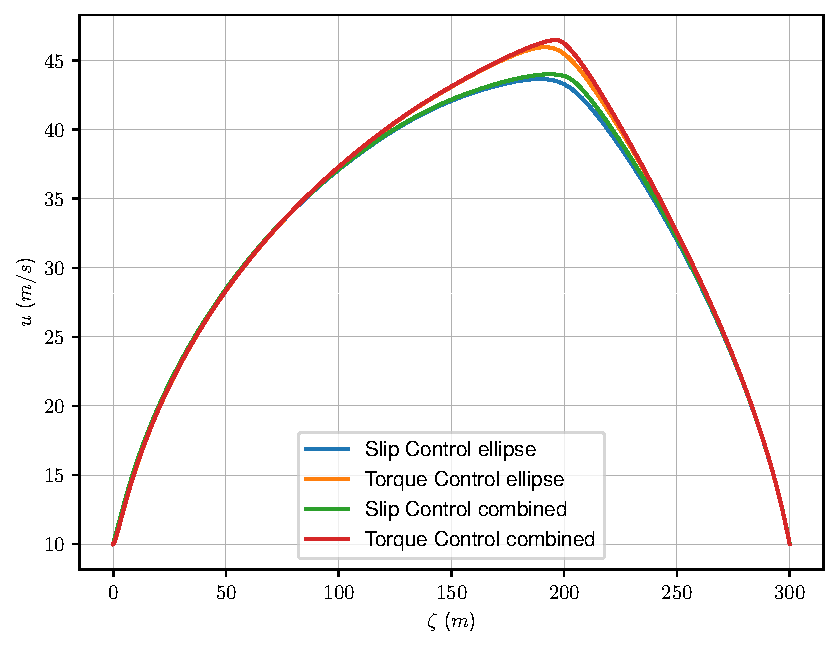
\includegraphics[width=\linewidth]{Straight/u_straight_confront.pdf}
        \caption{Longitudinal velocity}
        \label{fig:Straight1a}
    \end{subfigure}%
    \begin{subfigure}{0.5\linewidth}
        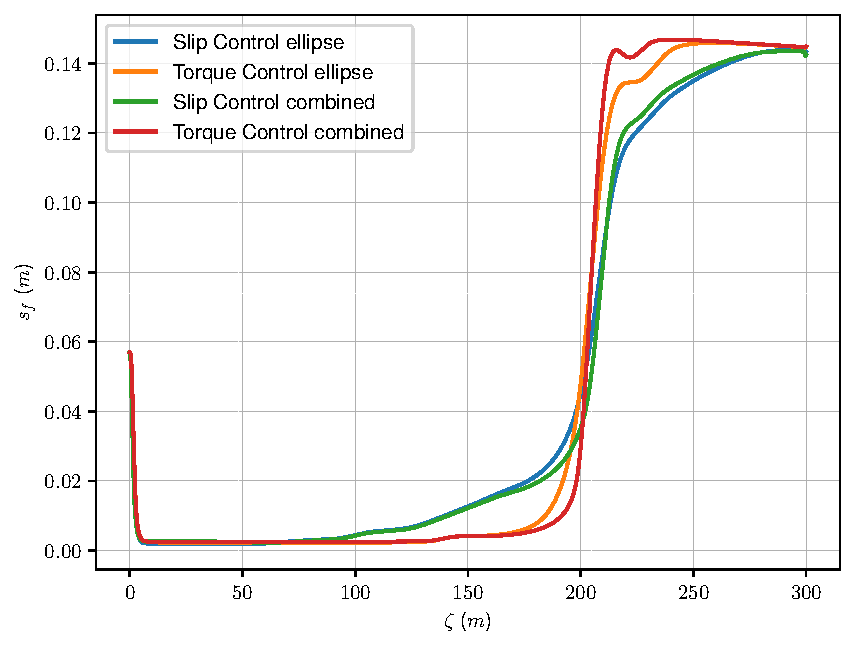
\includegraphics[width=\linewidth]{Straight/s_f_straight_confront.pdf}
        \caption{Front suspension deformation}
        \label{fig:Straight1b}
    \end{subfigure}
    \caption{Confront of result in straight running}
\end{figure}
%
%
\begin{figure}[t]
    \begin{subfigure}{0.5\linewidth}
        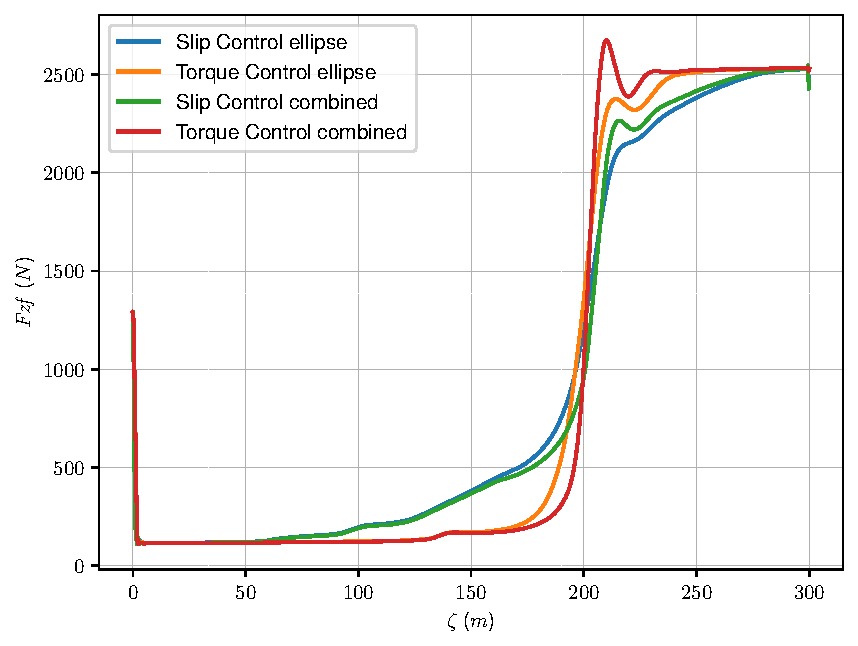
\includegraphics[width=\linewidth]{Straight/Fzf_straight_confront.pdf}
        \caption{Front}
        \label{fig:Straight2a}
    \end{subfigure}%
    \begin{subfigure}{0.5\linewidth}
        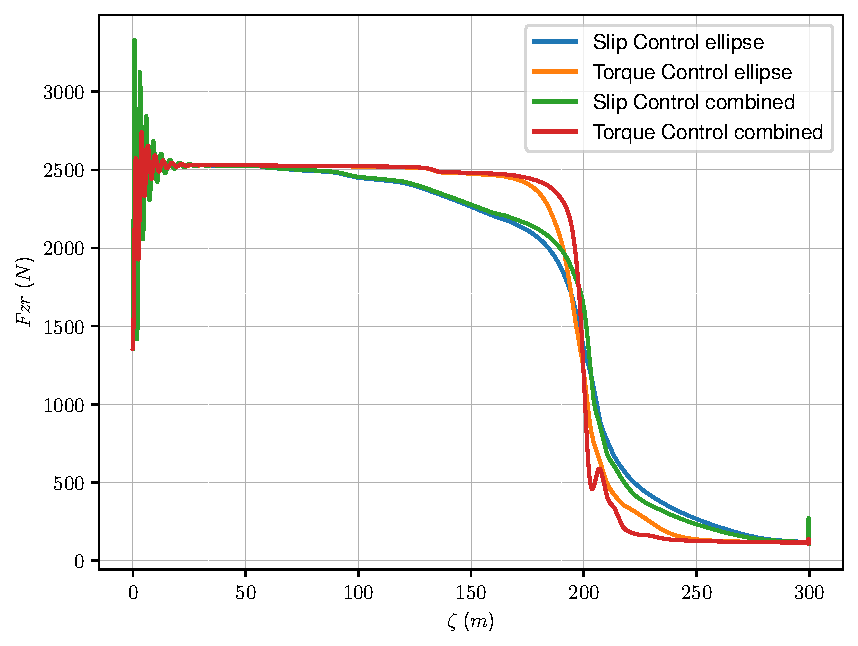
\includegraphics[width=\linewidth]{Straight/Fzr_straight_confront.pdf}
        \caption{Rear}
        \label{fig:Straight2b}
    \end{subfigure}
    \caption{Vertical forces in straight running}
\end{figure}
%
%
The results are the one expected as shown in the next figures. It is important to highlight that the slips control models have an exact solution which is the well known bang-bang as reported also by Leonelli and Limebeer. \cite{leonelli2019optimal}\\ 
The ellipse and the combined model produce almost the same behaviour. In fact they have a velocity peak that is almost identical (figure \ref{fig:Straight1a}). On the other hand, there is a small difference between the model controlled in torque and the ones controlled in slips. In fact, since the slip control neglect almost a lot of dynamical terms depending on the angular acceleration of the wheel we have a small difference.\\
In figure \ref{fig:Straight1b} it is clear that in all models there is a strong and fast load transfer. In fact, the motorcycle reach almost wheelie condition. It can be seen both from figure \ref{fig:Straight1b} and figures \ref{fig:Straight2b}-\ref{fig:Straight2b}. It is clear how, from the steady state distribution of masses, the front contact become almost non existent. In fact it reaches rapidly the limit imposed of the minimum load. In this condition the front wheel have zero authority in the control. Therefore if the vehicle is unsymmetrical some instabilities may arise. In real life those are compensated by the motion of the driver. The rear wheel, instead, is rapidly loaded and can exert a much higher force. It is clear that the torque control produce a manoeuvre that is definitely more aggressive, while the slip controls have a smother transition.
%
\begin{figure}[!ht]
    \begin{subfigure}{0.5\linewidth}
        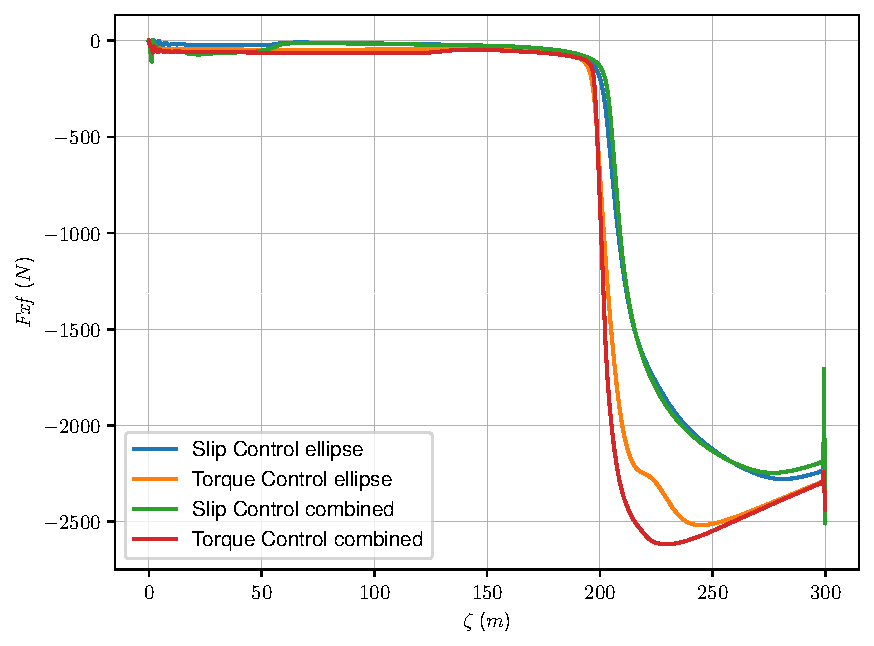
\includegraphics[width=\linewidth]{Straight/Fxf_straight_confront.pdf}
        \caption{Front}
        \label{fig:Straight3a}
    \end{subfigure}%
    \begin{subfigure}{0.5\linewidth}
        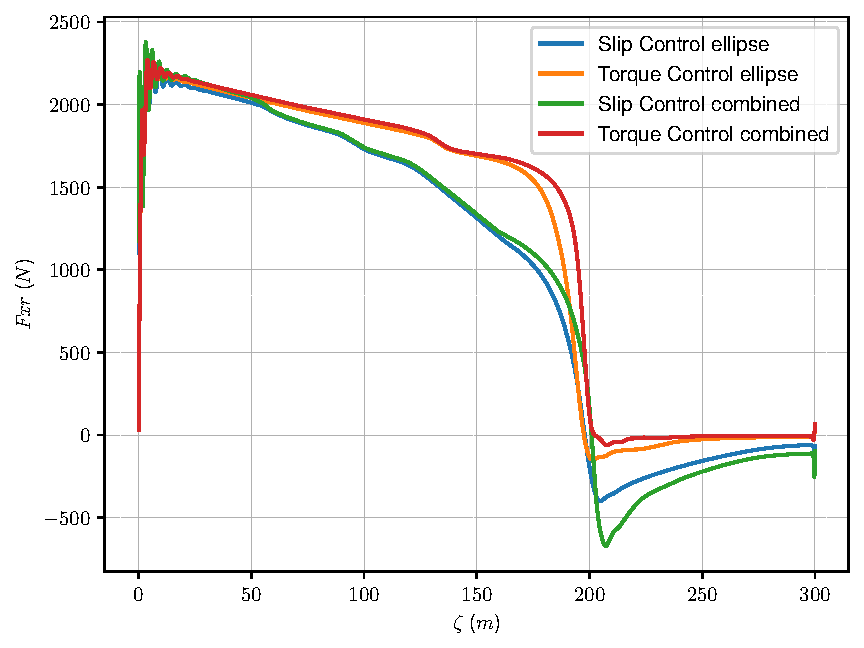
\includegraphics[width=\linewidth]{Straight/Fxr_straight_confront.pdf}
        \caption{Rear}
        \label{fig:Straight3b}
    \end{subfigure}
    \caption{Longitudinal forces in straight running}
\end{figure}
%
\\
As highlighted from figure \ref{fig:Straight3a} and \ref{fig:Straight3b} the motorcycle instantly produce a trust at rear wheel that decrease over the track until the point in which the motorcycle brakes. There is a strong difference between torque control and slip control. In fact, slip controlled model brakes with both wheels exploiting both wheels to their peaks of adherence. This is was somehow expected from the above figures.\\
At a close look one can appreciate that torque controls models have insignificant rear vertical load in braking condition. From the magic formula one can trivially see that with zero vertical load the maximum force is zero.\\
Another important aspect is the torque applied at the rear wheel. As highlighted in figure \ref{fig:StraightTorque} the torques in all four models respects the limit imposed by the maximum performance of the internal combustion engine. Moreover, in the first part is clear how the torque change from the low value of the steady state to the maximum exert by the tyre. In fact in this particular region the motorcycle is not using the full capability of the control. This particular behaviour is called partializing. \\
Before the braking point all models reach the performance limit. Again in braking condition is clear that slip control take advantage of both wheels while the torque braking is limited.\\
%
\begin{figure}%[!ht]
    \centering
    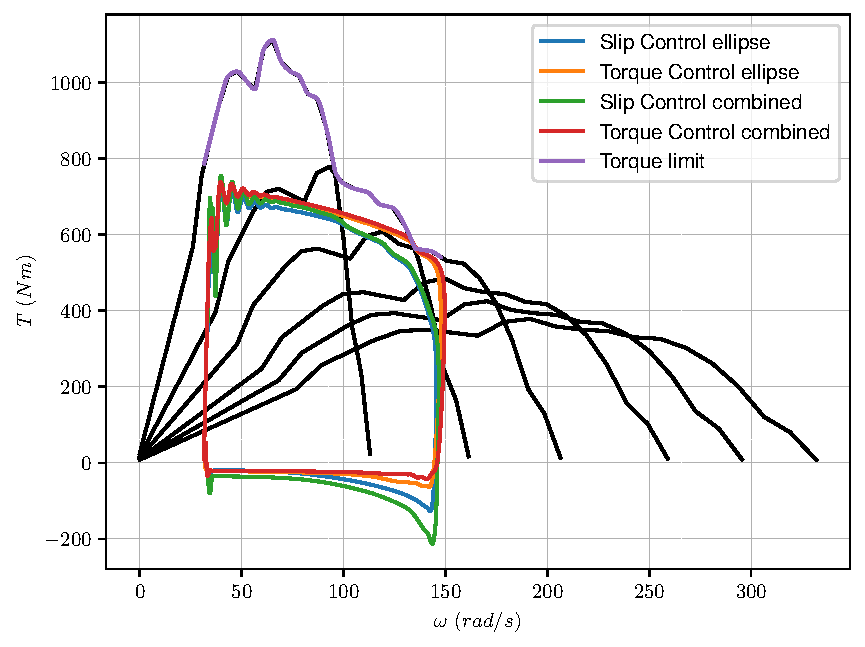
\includegraphics[width=0.8\linewidth]{Straight/Torque_straight_confront.pdf}
    \caption{Rear torque in straight running}
    \label{fig:StraightTorque}
\end{figure}
%
%